\section{Validation with Data from Photon Detector System Prototypes}
\label{sec:dp-pds-prototypes}

\subsection{Design Similarities and Differences Between Prototypes and Far Detector System}
The \dword{lar} \dword{tpc} \dword{dp} proposed technology is the result of years of R\&D. From small-scale chambers to the \dword{dune} module, many prototypes have been constructed, each with some design modifications and optimizations. 
Relevant to the \dword{pds} itself, the \dword{wa105}, operated at CERN in 2017, the \dword{pddp}, to be commissioned in 2019 and the \dword{dune} far detector module similarities and differences will be described here.

The first tonne scale dual phase \dword{lar} \dword{tpc} demonstrator has taken cosmic data between June and November \num{2017} at CERN. 
Located \SI{1}{m} below the charge collection plane, underneath the cathode and a ground protection grid, the photon detection system consisted of five \dwords{pmt} (Hamamatsu R5912-MOD20, described in more detail in Sec.~\ref{sec:dp-pds-selection-procurement}) evenly distributed along the 3$\times$1~m$^2$ area (one \dword{pmt} every \SI{50}{cm}). The demonstrator was considered as an opportunity to test different \dword{pds} designs, in particular in terms of \dword{tpb} coating and front-end electronics. Three \dwords{pmt} had the \dword{tpb} coating applied with evaporation directly onto their windows, whereas for the other two, the \dword{tpb} was deposited on a \SI{4}{\mm} thick transparent Plexiglass plate which was mounted on top of the \dwords{pmt}. 
While the latter solution has the advantage of being simpler and less risky to manipulate, it reduces the acceptance and possibly the efficiency due to the internal reflections between the \dword{tpb} and the Plexiglass surfaces. 

Two power supply polarities were used. Three \dwords{pmt} were equipped with a negative \dwords{hv} base, i.e. a negative bias voltage is applied to the photocathode and the anode is grounded. This system requires two cables: one for the \dwords{hv} system and one for the signal. A positive base was serving the other two \dwords{pmt}: a single cable positively biases the anode and carries the signal, and the cathode is grounded. The \dwords{hv} and the signal are then externally decoupled using a splitter, see Sec.~\ref{sec:fddp-pd-4.2}. The latter design has the advantages of reducing the number of feedthroughs and cables while also reducing the noise. Overall, four configurations were tested, as presented in Table~\ref{tab:dp-pds-311conf}. During the 3$\times$1$\times$1~m$^3$ operation, the \dwords{pmt} were operated at a rather uniform gain of around \num{e6} with a sampling of \SI{250}{MHz}.

\begin{dunetable}
[\dword{wa105} \dwords{pmt} configurations.]
{cccccc}
{tab:dp-pds-311conf}
{Configuration of the five \dwords{pmt} installed in the \dword{wa105}}
\dword{pmt} & Base & Coating & Voltage (kV) & Gain (\num{e6}) & Noise (ADC)\\
%\hline
1 & Negative & Coating & \num{-1.2} & 0.92$\pm$0.13 & \num{0.7} \\
2 & Negative & Plate   & \num{-1.2} & 1.01$\pm$0.12 & \num{0.7} \\
3 & Positive & Coating & \num{1.1} & 0.95$\pm$0.11 & \num{0.4} \\
4 & Positive & Plate   & \num{1.1} & 1.26$\pm$0.15 & \num{0.4} \\
5 & Negative & Coating & \num{-1.2} & 1.33$\pm$0.15 & \num{0.8} \\
%\hline
\end{dunetable}

In \dword{pddp}, 36 \dwords{pmt} are installed \SI{6}{\m} below the collection plane, again underneath the cathode and a ground protection grid. The \dword{pmt} density is lower compared to the demonstrator. Their positioning along the \SI{36}{m$^2$} area was optimized with simulations. The number of the \dwords{pmt} is higher around the center of the active volume and lower near the field cage borders. This positioning maximizes the amount of light collection from cosmic rays.

Following the evaluation of the demonstrator configurations, the \dword{tpb} was directly evaporated onto the \dword{pmt} windows and the electronic base was chosen to have positive polarity. This configuration maximizes the collection efficiency, and reduces both the number of cables and the electronic noise. 

For \dword{dune} \dword{fd} \dword{pds}, \dword{tpb} will be directly coated onto the \dword{pmt} windows and positive biasing scheme will be implemented. As the aspect ratio between cathode size and drift distance is larger compared to \dword{pddp}, the amount of light loss by absorption on the field cage is expected to be smaller. Therefore, the \dword{dune} \dword{fd} \dword{pds} layout is foreseen to be uniform, with \dwords{pmt} on a regular lattice with \SI{1.02}{m} spacing. On the other hand, light attenuation due to absorption in the \lar itself will be larger in the \dpmod.

%%%%%%%%%%%%%%%%%%%%%%%%%%%%%%%%%%%%%%%%%%%%%%%%%%%%%%%%%%%%%%%%%%%%

\subsection{Photon Detector Simulation}
For a \dword{mip}, an energy of about \SI{2}{\MeV/\cm} is deposited in \dword{lar}. 
Through decays of excited argon states and ion recombination, about \num{40000} scintillation photons are emitted per \si{\MeV} deposited at null drift field. At the nominal drift field of \SI{500}{\V/\cm}, this amount reduces down to about \num{24000} photons per \si{\MeV} as the recombination process is weaker. 
This signal, known as S1 (see Sec.~\ref{sec:dp-pds-overview}), is common to the single and dual phase technologies.

In the gas layer of the dual phase design, the electrons are amplified through Townsend avalanche in the \dword{lem} holes, and lead to an electroluminescence signal called S2 (see Sec.~\ref{sec:dp-pds-overview}). The electroluminescence gain, $G_{EL}$, i.e. the number of photons produced per electrons crossing the liquid-gas interface, depends on the voltages applied to the \dword{lem}. The S1 and S2 signals have similar characteristics in terms of wavelength and time constants. 

Due to different mechanisms during photon propagation (Rayleigh scattering, absorption by impurities in the \lar or by elements constituting the detector), only about a \num{1e-3} fraction of the photons produced in the \lar active volume reaches the \dword{pmt} photo-cathodes. The direct simulation of the large number of photons generated for each track crossing the active volume would require a considerable amount of CPU power and time. Profiting from the fact that the photon emission is isotropic and the detector is uniform and symmetric, we have decided to generate the photon propagation in the detector in a dedicated Geant4 simulation only once.

The active volume is divided into voxels, and a large amount of photons are isotropically generated at the center of each voxel. 
The amount of photons collected by each \dword{pmt}, and the propagation time is stored and later parametrized. For long voxel-\dword{pmt} distances (typically larger than \SI{1}{\m}), a landau function is well suited to reproduce the time distribution.
The detection probability, called visibility, the landau parameters (MPV, $\sigma$) and the minimal time needed by the photon to reach the \dword{pmt} are stored in light maps for all voxel-\dword{pmt} combinations. When a track is generated in the standard dual phase \dword{larsoft} simulation toolkit, for each step of the track, the light map is looked up to assign the amount of photons to be collected at each \dword{pmt}. The \dword{larsoft}-based preliminary light maps for \dword{pddp} and for \dword{dune} \dword{fd} have been created. As an example, the total light yield per MeV deposited in \dword{pddp} is shown in Fig.~\ref{fig:dppd_protodunedp_light_yield}.

\begin{dunefigure}[Expected light yield in \dword{pddp}]{fig:dppd_protodunedp_light_yield}{Expected light yield (in PEs/MeV) in \dword{pddp} as a function of spatial (x,z) position in the \dword{lar} active volume, and averaged along the y-axis. The z-axis is parallel to the drift direction.}
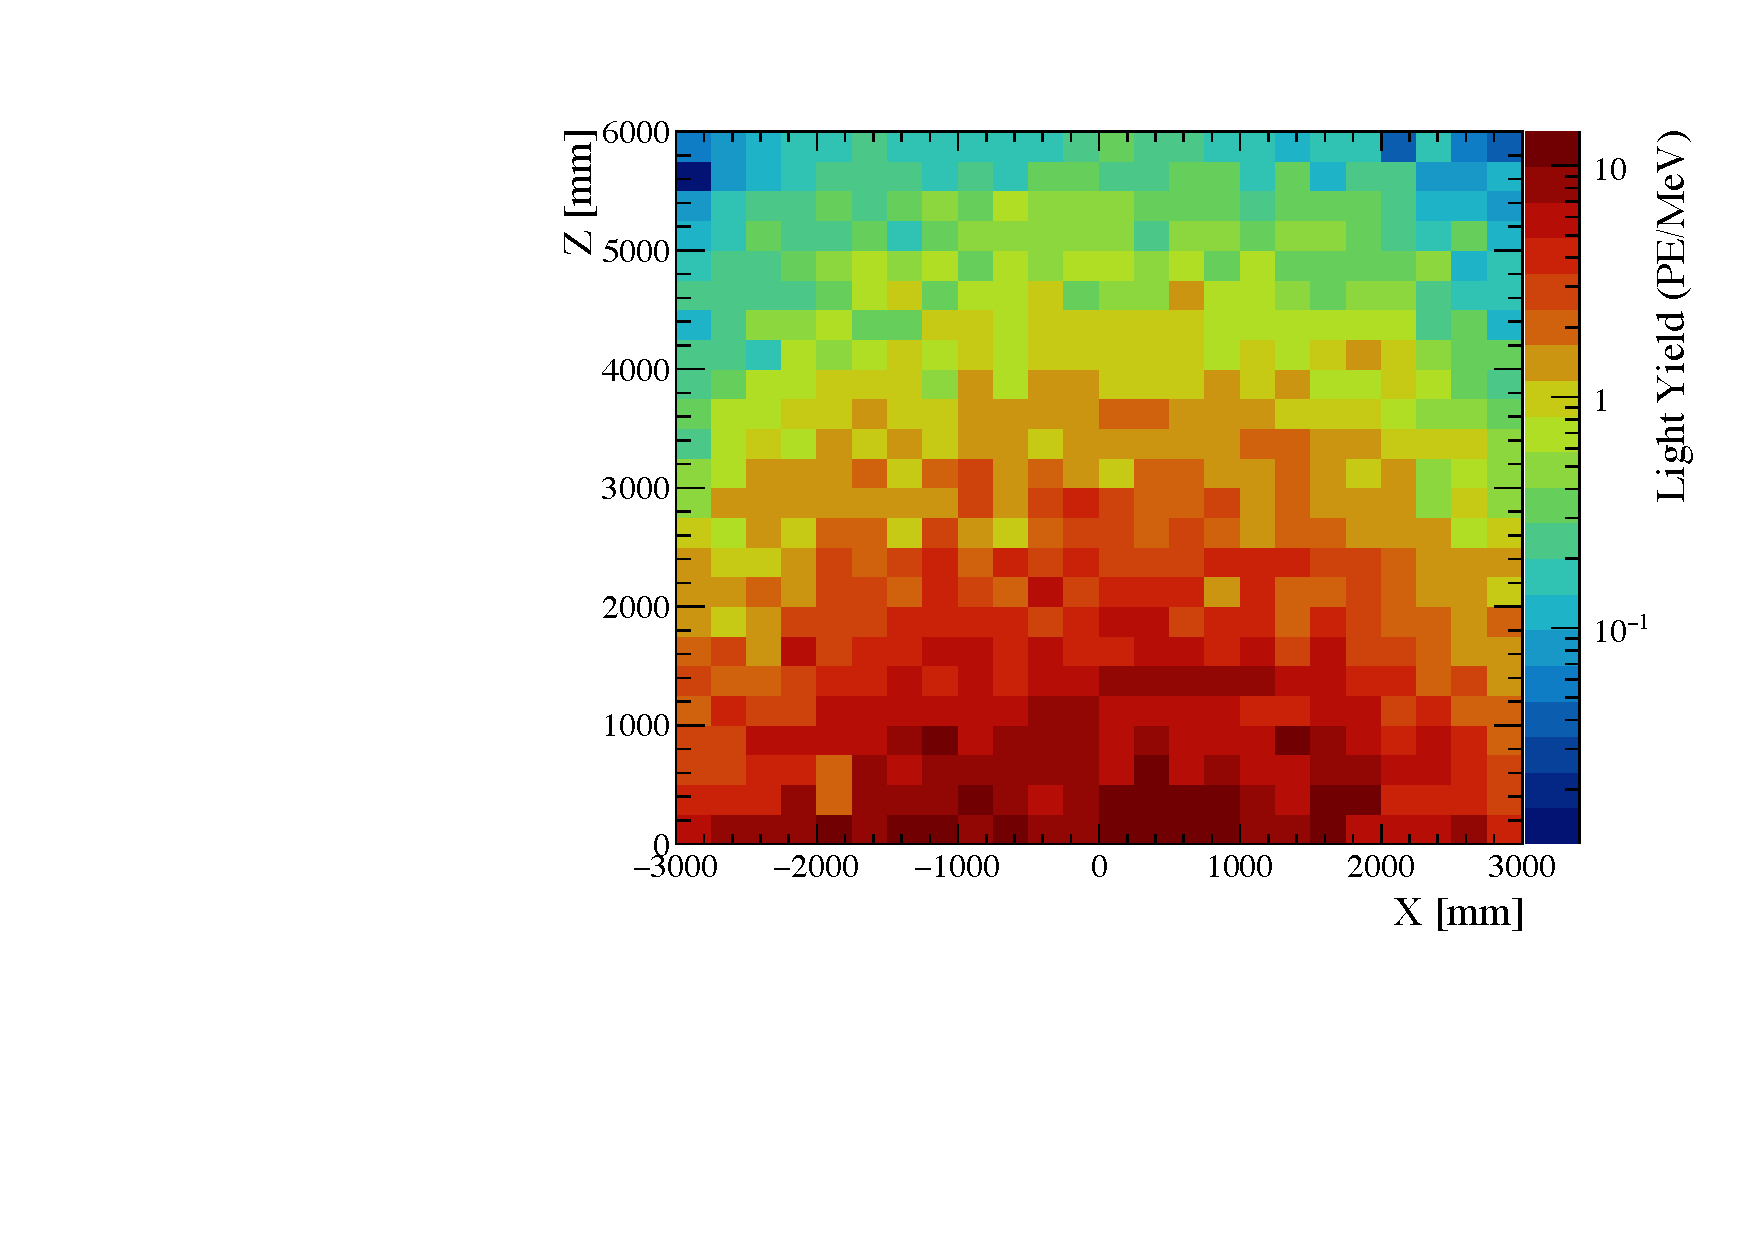
\includegraphics[width=0.6\textwidth]{graphics/dppd_protodunedp_light_yield.pdf}
\end{dunefigure}

%%%%%%%%%%%%%%%%%%%%%%%%%%%%%%%%%%%%%%%%%%%%%%%%%%%%%%%%%%%%%%%%%%%%

\subsection{\dword{wa105} Light Data Results and Simulation Validation}

\fixme{The \dword{wa105} simulation to be validated in this section needs to change from LightSim to \dword{larsoft}}

The analysis of the data taken during the \dword{wa105} operation provides the first handle on the validation and improvement of the light simulation developed so far. 
The active volume of the demonstrator ($3\times1\times1$~m$^3$) is rather small with respect to the assumed Rayleigh scattering length of $L_{ray} = 55$~cm. 
As a consequence, the light absorbed by elements of the detector (such as the field cage, \dword{lem} or cathode) may become a dominant factor.
Hence, the light maps were created with particular care given to the precision in the reproduction of the demonstrator's geometry.

Two triggering schemes were used during the \dword{wa105} operation.
The first was provided by an external muon tagger, the Cosmic Ray Tagger (CRT), to record horizontal muons. The CRT was made of plastic scintillator planes located on each side of the detector.
The second was performed by the \dwords{pmt} themselves, requiring that the five sensors recorded sufficient amount of light in coincidence. In this configuration, a higher number of vertical muons were recorded, as well as showers.

In the CRT trigger condition, a rough track reconstruction is possible as the CRT provides coordinate information with 11~cm$^2$ resolution. Hence, even without the charge information, like for data taken at null field, it is possible to select muon-like tracks and to retrieve the shortest distance between the track and each \dword{pmt}. A schematic drawing of the \dword{wa105} detector is presented in Fig.~\ref{fig:pd-pds-311schema}, along with the relevant track parameters.

\begin{dunefigure}[\dword{wa105} schematic drawing]{fig:pd-pds-311schema}{Schematic view of the \dword{wa105}. 
The fiducial volume is represented in gray and is limited from the collection plane area to the cathode. In yellow, the active volume is presented. Its volume is defined by the collection plane, the field cage to the tip of the \dwords{pmt}. A track that would be detected by the CRTs is shown, with its minimum distance to \dword{pmt} 3 is shown in red.}
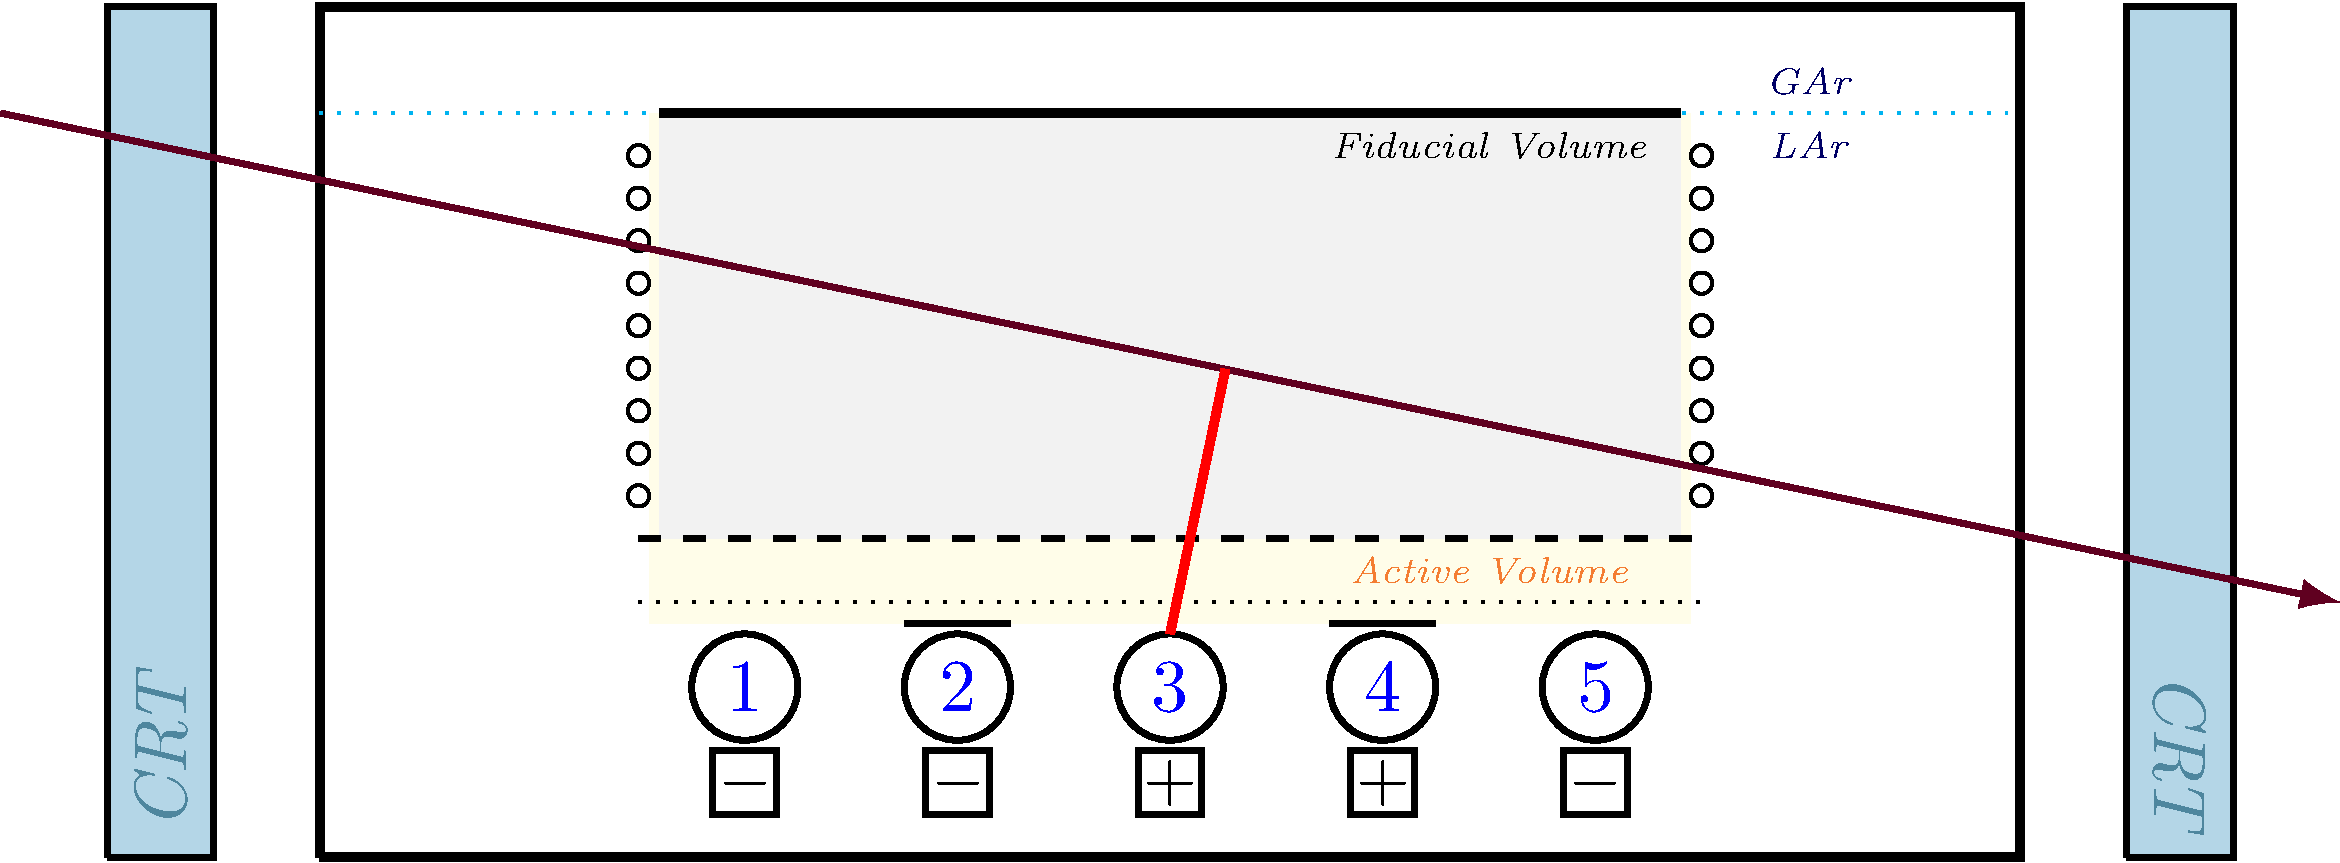
\includegraphics[width=0.8\textwidth]{graphics/dppd_7_2}
\end{dunefigure}

Using data taken at null field in CRT triggering mode, a selection of muon-like tracks is performed. It is further required that the tracks cross the active volume for distances longer than \SI{3.1}{\m}. 
The S1 charge collected by each \dword{pmt} is calculated by integrating the ADC values in a \SI{1}{\us} window starting from the S1 peak, and this charge value is then converted into the number of detected photoelectrons (PEs) using the calibrated \dword{pmt} gains given in Tab.~\ref{tab:dp-pds-311conf}.

\begin{dunefigure}[Charge Collected in \dword{wa105} vs MC]{fig:dp-pds-311charge}{ Charge collected by the \dwords{pmt} in a \SI{1}{\us} window containing the S1 peak for muon-like tracks triggered by the CRT panels. The data is shown with blue squares and the simulation with red circles. The distributions are normalized to unity for clarity. Preliminary results.}
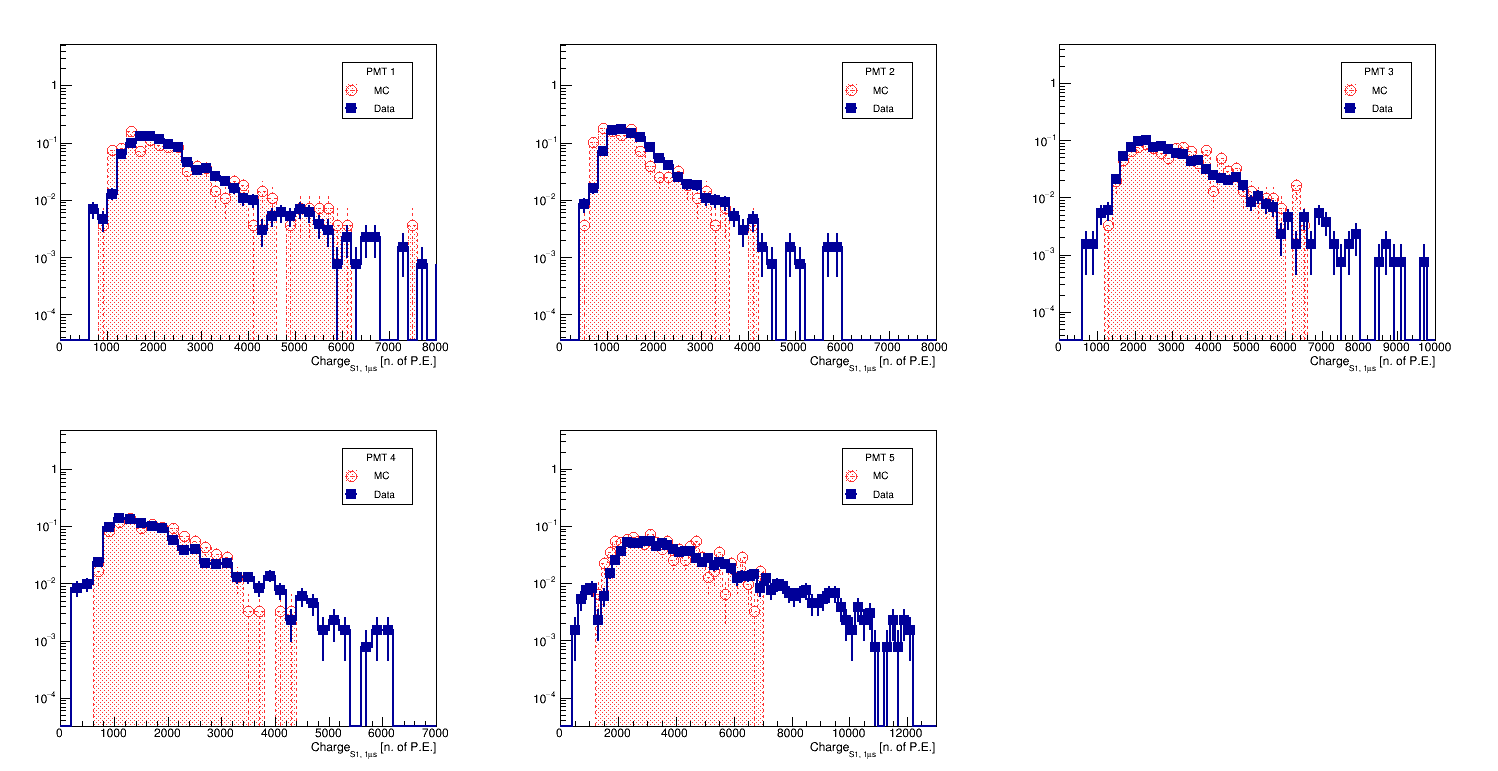
\includegraphics[width=0.95\textwidth]{graphics/dppd_7_3.png}
\end{dunefigure}

In the simulation, \SI{4}{\GeV} muons are generated from one CRT panel to the other with data-driven kinematics. The number of PEs collected by each \dword{pmt} is generated according to the light maps. A selection on the minimum amount of light recorded by all \dwords{pmt} in order to suppress spurious triggers is used in the data analysis and does not apply to the case of MC. Additionally, the requirement that the \dword{pmt} signal does not saturate the readout is implemented only for the data analysis and not MC. A comparison of the number of PEs collected in data and in MC is presented in Fig.~\ref{fig:dp-pds-311charge}. The result shows a good agreement between data and MC.

\fixme{Give more details about why \dword{pmt} saturation in \dword{wa105}, and why this is not worrisome in \dpmod?}

\begin{dunefigure}[Charge Collected vs track-PMT shortest distance]{fig:dp-pds-311profile}{Profile histograms of charge collected as a function of the track-PMT distance. The data is in blue squares, the simulation in red circles. Preliminary results.}
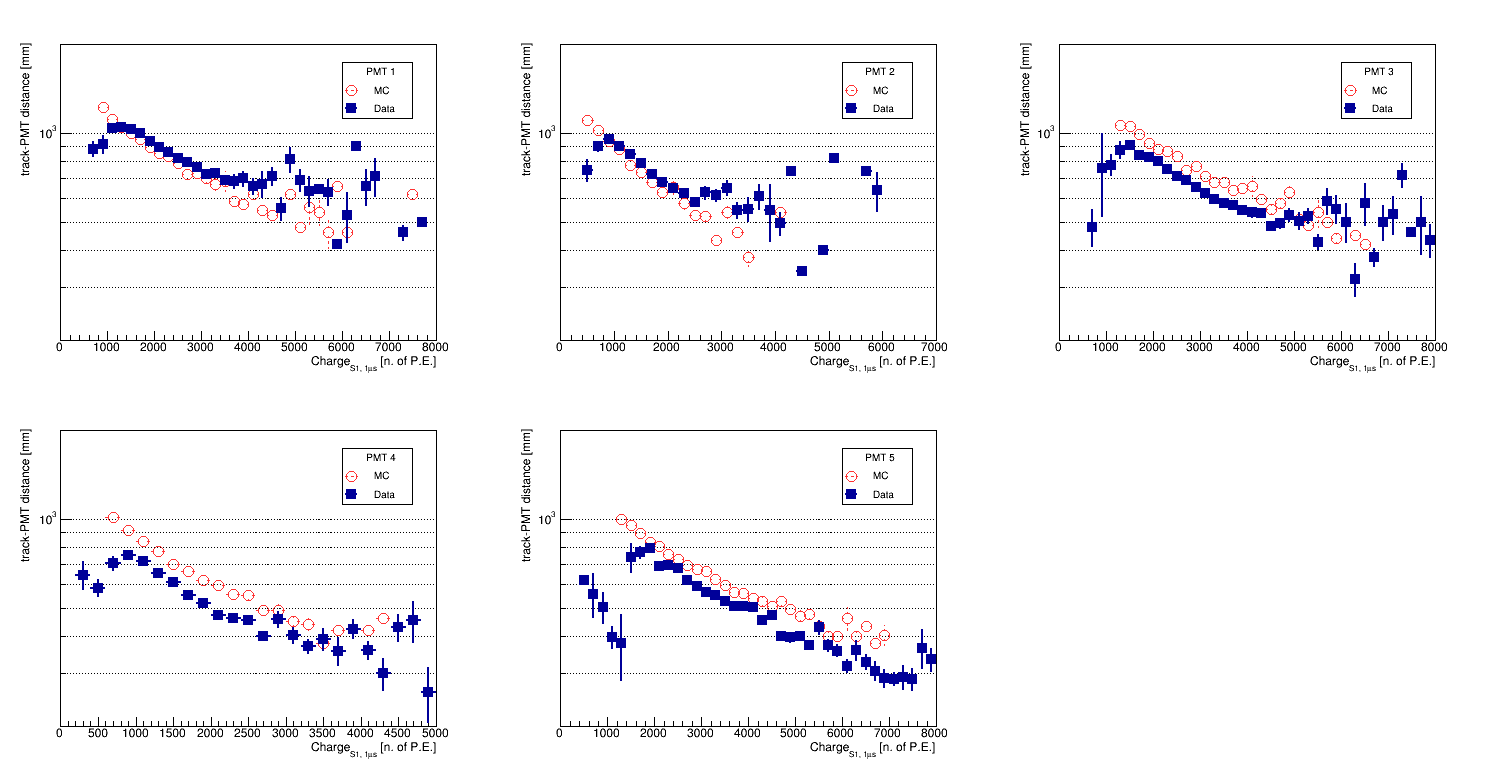
\includegraphics[width=0.95\textwidth]{graphics/dppd_7_4.png}
\end{dunefigure}

\fixme{This is rather distance vs charge. Is it possible to swap the x and y axis and reproduce the plots?}

The amount of PEs collected per \dword{pmt} depends strongly on the shortest track-PMT distance. Many factors can affect the amount of charge collected, the dominant one being the scattering length, also known as the Rayleigh scattering. This quantity is still subject to debate among the \dword{lar} community as its measurement is fairly complicated. Current estimates of the scattering length range from \SI{20}{\cm} to \SI{1}{\m}.
In the \dword{wa105} simulation, the scattering length was set to L$_{ray}$ = \SI{55}{\cm}.
Figure~\ref{fig:dp-pds-311profile} shows the charge collected as a function of the shortest track-PMT distance in the form of profile histograms. The overall trend is very similar for data and MC, also across all the \dwords{pmt}. However, the profile histogram slopes indicate that the assumed scattering length in MC could be better tuned to reproduce the data, e.g. towards larger values of the Rayleigh scattering length.

%%%%%%%%%%%%%%%%%%%%%%%%%%%%%%%%%%%%%%%%%%%%%%%%%%%%%%%%%%%%%%%%%%%%

\subsection{Preliminary (or Prospects for) ProtoDUNE-DP Light Data Results}

\fixme{Add lessons learned from \dword{pddp} installation and commissioning here?}